% Created 2017-11-25 Sat 21:30
\documentclass[11pt]{article}
\usepackage[utf8]{inputenc}
\usepackage[T1]{fontenc}
\usepackage{fixltx2e}
\usepackage{graphicx}
\usepackage{longtable}
\usepackage{float}
\usepackage{wrapfig}
\usepackage{rotating}
\usepackage[normalem]{ulem}
\usepackage{amsmath}
\usepackage{textcomp}
\usepackage{marvosym}
\usepackage{wasysym}
\usepackage{amssymb}
\usepackage{hyperref}
\tolerance=1000
\usepackage{minted}
\usepackage{fancyhdr}
\setcounter{secnumdepth}{-1} 
\pagestyle{fancy}
\fancyhead{} 
\rhead{\textit{Michael Laufer}}
\lhead{\textit{Numerical Methods Fall 2017, HW6}}
\small

\author{Michael Laufer}
\date{\today}
\title{HW4 Numerical Methods Fall 2017}
\hypersetup{
  pdfkeywords={},
  pdfsubject={},
  pdfcreator={Emacs 25.3.1 (Org mode 8.2.10)}}
\begin{document}

\maketitle
\section{ADI Iterative Scheme - 4th Order Poisson}
\label{sec-1}
\subsection{Problem}
\label{sec-1-1}
Given the Poisson equation:
\[
\frac{\partial^{2} \phi}{\partial x^{2}} + \frac{\partial^{2} \phi}{\partial y^{2}} = S_{\phi}
\]
Where $S_{\phi}$ is defined as:
\[
S_{\phi} = 50000 \exp \left[ -50 \left{ \left( 1 - x )^{2} + y^{2} \right} \right] \cdot \left[ 100 \left{ \left( 1 - x \right)^{2} + y^{2} \right} -2 \right]
\]
Derichlet boundary conditions are given as functions defined on the unit square domain boundary. \\
The system has an analytical solution given by:
\[
\phi \left( x,y \right) = 500 exp \left( -50 \left{ \left( 1 - x \right)^{2} +y^{2} \right} \right) + 100x \left( 1 - y \right)
\]

Using a second order central differencing equation leads to the following scheme, which we have discussed at length in previous assignments.
\[
-\left( \frac{2}{ \left( \Delta x \right) ^{2}} + \frac{2}{ \left( \Delta y \right) ^{2}} \right) \phi_{i,j} + \frac{1}{ ( \Delta x )^{2} } \phi_{i+1,j} + \frac{1}{ ( \Delta x )^{2} } \phi_{i-1,j} + \frac{1}{ ( \Delta y )^{2} } \phi_{i,j+1} + \frac{1}{ ( \Delta y )^{2} } \phi_{i,j-1}=S_{i,j}
\]

This equation is solved at each node leading to a system of $n_{x}n_{y}$ equations. 
We will be examining a number of iterative methods to solve the system of equations. 
In particular, the system will be solved using the following methods:
\begin{enumerate}
\item Jacobi Method
\item Gauss-Seidel Method
\item Method of Steepest Descent (MSD)
\item Conjugate Gradient Method (CG)
\item Conjugate Gradient Squared Method (CGS)
\end{enumerate}


\subsection{Jacobi Method}
\label{sec-1-2}
In this method, the equations are rearranged such that all terms except the the diagonal term are transposed to the right-hand side of the equation. Additionaly the entire equaiton is divided byt he diagonal coeffcient yeilding the scheme:
\[
\phi_{k}^{n+1} = \frac{Q_{k} - \sum\limits_{j=1 \\ j \neq k}^{N_{nb,k}} a_{j} \phi_{j}^{n}}{a_{k}}
\]
In effect, values of $\phi$ are updated at each iteration in a totally explicit manner, where all reference values are taken as values from the previous iteration. It is important to note at this point that due to this fact, values can be updated in a parallel or vectorized manner, where all values in the solution array are updated concurrently. The computational costs of this will be explored later on in this assignment.

\subsection{Gauss-Seidel Method}
\label{sec-1-3}
This method is very similiar to the Jacobi method, but values that have been just computed in the current iteration are used where possible. This allows for more up to date data to be used compared to Jacobi, and thus allows boundary conditions to propogate at a faster rate thorughout the domain leadign to a smaller number of iterations to acheive convergence than Jacobi. The Gauss-Seidel scheme is defined as:
\[
\phi_{k}^{n+1} = \frac{Q_{k} - \sum\limits_{j=1 \\ j \neq k}^{N_{nbu,k}} a_{j} \phi_{j}^{n+1} - \sum\limits_{j=1 \\ j \neq k}^{N_{nb,k} - N_{nbu,k} } a_{j} \phi_{j}^{n} }{a_{k}}      
\]
We can see here that values must be updated one by one, a process that cannot be parallelized or vectorized. We can infer here that this method will require a double for loop to loop over all the elements in the domain. In a dynamically typed language such as python, this in general leads to a slow computation.  In order to accelrate this type of solver, Numba is employed, bringing C-like performance (this has been coveraed at length in HW3). Solving times of both an accelerated and pure-Python version of Gauss-Seidel will be compared to a vectorized version of the Jacobi method. 

\subsection{Method of Steepest Descent (MSD)}
\label{sec-1-4}
This method is different than other methods explored up to now. This method solves an optimation problem of the following function:
\[
f(\phi_{1}, \phi_{2},..... \phi_{K}) = \frac{1}{2} [\phi]^{T} [A] [\phi] - [Q]^{T} [\phi] +c
\]
Assuming a symetric $A$ matrix, which is correct in our Poisson eqaution, taking a gradient of this function and equating to zero (finding a local optimum of the function)  leads to:
\[
\grad f = [A][\phi] - [Q] = 0
\]
Which is exactly the eqation we are trying to solve.
Additionally, we can show that the residual vector is equal to the negative of the gradient vector, which as we know points in the direction of the steepest decent/ascent of the function.  
Thus starting from an initial guess and travelling in the direction of the gradient vecotor (negative residual vector) leads us to the optimum, or solution to the given problem. As a consequnce, subsequent search directions are orthogonal to each other.

The book outlines a method to do just this on page 149, but it is pertinent to note that the algorithm shown utilizes a series of double and single for loops in each iteration. The code actually implemented has no for loops and is purely a vectorized operation (see appendix for implementation). 

\subsection{Conjugate Gradient Method (CG)}
\label{sec-1-5}
The Conjugate Gradient method  is very similiar to the Method of Steepest Descent, but instead of searching in a stair-step pattern (due to the orthoganility of successive search directions in MSD), a linear of combination the old direction vector and newly computed direction vector is used. This porduces a more smoothly convergent computation, generally leading to lower iteration counts. This too has been implemented in a fully vectorized manner, acclerating computational time.

\subsection{Conjugate Gradient Squared Method (CGS)}
\label{sec-1-6}
Lastly, the Conjugate Gradient Squated method circumvents the limitation of the MSD and CG method where the $A$ matrix must be symemtric, a limitation that makes those methods unusable in many enginnering calculations. Interestingly, this method has been shown to yield the exact solution to a problem in no more than $N_{x}N_{y}$ iterations. As with the other methods except for Gauss-Seidel, this mehod has been implemented in a vectorized manner. 




\subsection{Convergence Criterion}
\label{sec-1-7}
Convergence is monitored with the use of the $L^{2}Norm$ defined as:
\[
R2 = \sqrt{ \sum_{k=1}^{K} ( R_{k})^{2} }
\]
where:
\[
R_{k}^{n} = Q_{k} -a_{k} \phi_{k}^{n} - \sum_{j=1 \\ j \neq k}^{N_{nb,k}}  a_{j} \phi_{j}^{n}  
\]

For a 2nd order scheme this computation involves iterating over every node and accessing 4 neighboring nodes. A better approach is to use vectorized code, and notice that matrix addition can be used to replace the expensive double for loop. This is illustrated in the following python snippet.
\begin{minted}[]{python}
def l2norm(phi, S, dx2, dy2):
    Rk =S[1:-1,1:-1] +((2/dx2) + (2/dy2))*phi[1:-1,1:-1] - (1/dx2)*phi[1:-1,2:] \
- (1/dx2)*phi[1:-1,0:-2]  - (1/dy2)*phi[2:,1:-1] - (1/dy2)*phi[0:-2,1:-1] 
    Rksquared = np.multiply(Rk,Rk)
    return (math.sqrt(Rksquared.sum()))
\end{minted}


\subsection{Results}
\label{sec-1-8}
All methods were solved till $l^{2}Norm$ fell below 10e-7.
Solution, and error contour plots are first plotted for the Jacobi method to show convergence to the exact solution. 

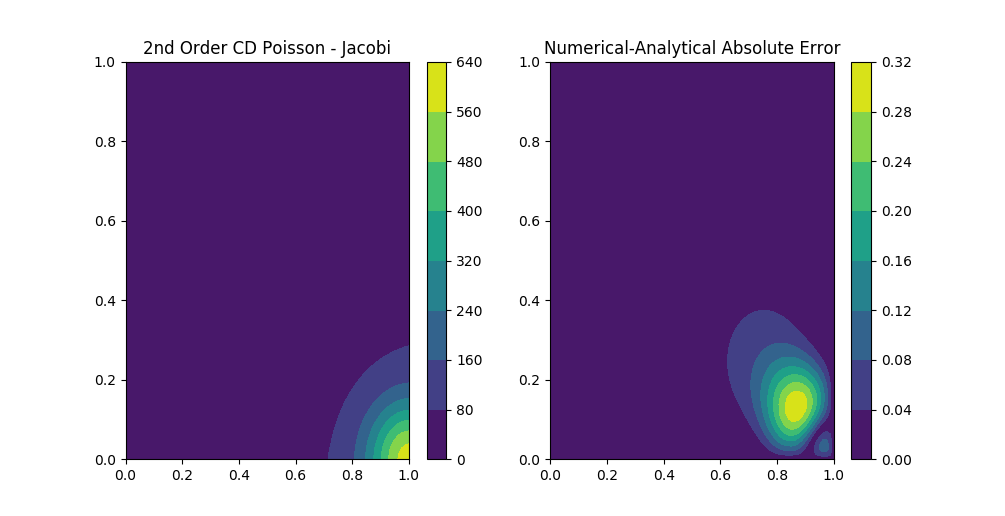
\includegraphics[width=12cm]{./figures/solution.png}

We can see that the iterative method solution agrees well with the analytical result.
A 3d plot of the solution is seen in the following figure:
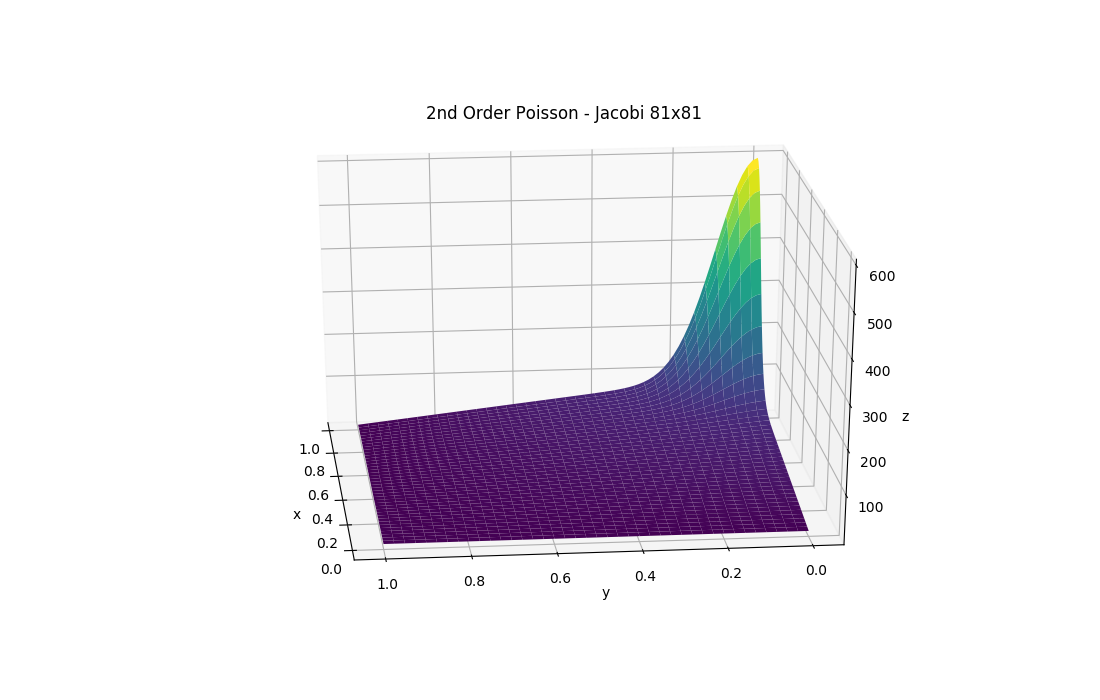
\includegraphics[width=12cm]{./figures/3d.png}

Residuals for all of the methods examined is given in the following figure:
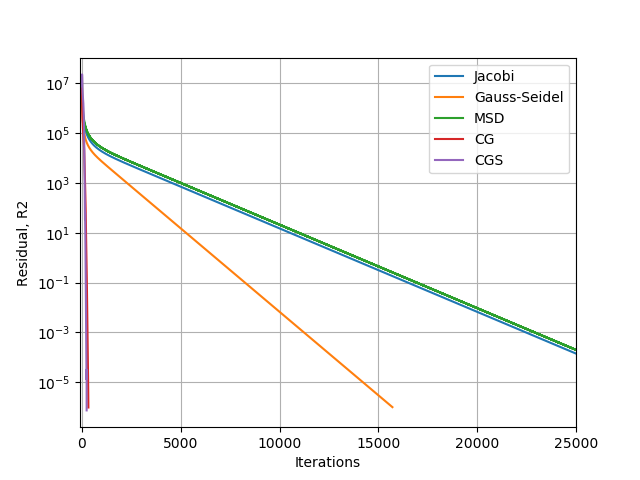
\includegraphics[width=12cm]{./figures/residual1.png}

Additionally focusing in on the two fastest methods, the CG method and CGS method gives:

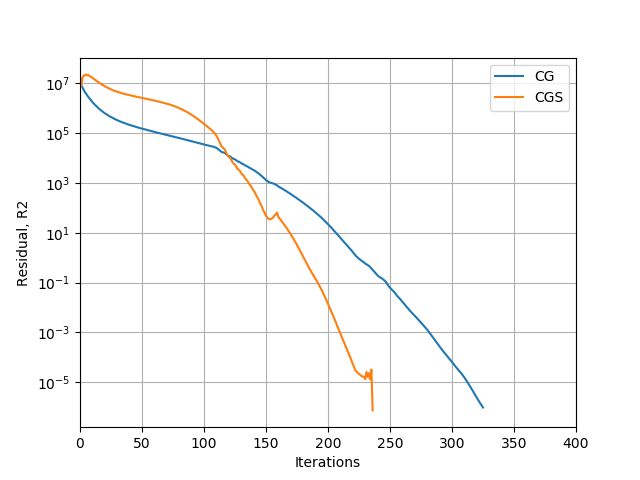
\includegraphics[width=12cm]{./figures/residual2.png}

The total number of iterations to the convergence of $l^{2}Norm$ below 10e-7 is tabulated in the following table:
\begin{center}
\begin{tabular}{ll}
\hline
Method & Iterations on 81x81 Grid\\
\hline
Jacobi & 31,419\\
Gauss-Seidel & 15,710\\
MSD & 32,860\\
CG & 325\\
CGS & 236\\
\hline
\end{tabular}
\end{center}


\subsection{Discussion}
\label{sec-1-9}
It is clear that the CG and CGS methods are by far the most efficient in regards to iterations to convergence. Additionally, similar to results in the book on page 157, the Gauss-Seidel solver solved around half the number of iterations, compared to the Jacobi solver. Interestingly, considering the MSD method is in the same family as both CG and CGS, the total number of iterations is even higher than the "naive" Jacobi method, this too is consistent with results in the book in example 3.8.   
When looking closely at the CG method vs the CGS method, we can see that the CGS method shows erratic performance at the onset of the computation, lagging behind CG. Shortly afterwards, the CGS method rapidly overtakes CG and converges mot rapidly to the solution.

As we have seen before, the number of iterations is not the whole picture, the total computation time is of most importance, especially in applied computations.  The computational time for all 5 methods, both with and without Numba acceleration can be observed in the following table. Note, that computations were performed on a Intel 2-core i5-4200U @ 1.6ghz base-clock with 4 GB of RAM.
\begin{center}
\begin{tabular}{lrll}
\hline
Method & Pure Python (Numpy) & Numba & Fastest Compared to Baseline\\
\hline
Jacobi & 7.47 & \textbf{6.53} & 78\%\\
Gauss-Seidel & 241 & \textbf{3.62} & 43\%\\
MSD & 9.27 & \textbf{8.29} & 100\%\\
CG & \textbf{0.144} & 1.07 & 1.7\%\\
CGS & \textbf{0.122} & 1.21 & 1.4\%\\
\hline
\end{tabular}
\end{center}

We fist see that due to the double for loop inherent in the pure python Gauss-Seidel method (which cannot be vectorized), the Jacobi method is over 4 times faster the GS method. But Numba is found to be able to  acclerate the Gauss-Seidel method by a factor of 65 and actually performs better than the highest performing Jacobi.  This shows both the power of vectorized code, but also the speed up possible with using a Just-In-Time (JIT) accelerator like Numba.  

We can also observe that the CG and CGS methods are actually fastest in their fully vectorized pure Python versions without Numba. Here Numba dramatically slows down the code due to the overhead involved with compiling the code. 

5 independent methods have been used to solve our original Poisson equation, and a large variance in number of iterations needed for convergence, and solving time is seen.

\newpage
\section{Appendix: Python Code}
\label{sec-2}
\begin{minted}[]{python}
import matplotlib.pyplot as plt
import numpy as np
import math
import time
from scipy.linalg import *
from numba import jit, prange
from mpl_toolkits.mplot3d import Axes3D
from matplotlib import cm


def l2norm(phi, S, dx2, dy2):
    Rk =S[1:-1,1:-1] +((2/dx2) + (2/dy2))*phi[1:-1,1:-1] \
- (1/dx2)*phi[1:-1,2:] - (1/dx2)*phi[1:-1,0:-2]  - (1/dy2)*phi[2:,1:-1] - (1/dy2)*phi[0:-2,1:-1] 
    Rksquared = np.multiply(Rk,Rk)
    return (math.sqrt(Rksquared.sum()))

def l2normMSD(phi, S, dx2, dy2):
    ny, nx = phi.shape
    Rk = np.zeros((ny,nx))
    Rk[1:-1,1:-1] = S[1:-1,1:-1] +((2/dx2) + (2/dy2))*phi[1:-1,1:-1] \
 - (1/dx2)*phi[1:-1,2:] - (1/dx2)*phi[1:-1,0:-2]  - (1/dy2)*phi[2:,1:-1] - (1/dy2)*phi[0:-2,1:-1] 
    Rksquared = np.multiply(Rk,Rk)
    R2sum = Rksquared.sum()
    norm = (math.sqrt(Rksquared.sum()))
    return (R2sum, Rk, norm)
@jit
def jacobistep(phi,S, dx2, dx):
    phin = phi.copy()
    phi[1:-1,1:-1] = (S[1:-1,1:-1] - (1/dy2)*phin[0:-2,1:-1] \
- (1/dy2)*phin[2:,1:-1] - (1/dx2)*phin[1:-1,0:-2] - (1/dx2)*phin[1:-1,2:])/(-((2/dx2) + (2/dy2)))
    return(phi)

@jit
def gaussstep(phi,S, dx2, dx):
    phin = phi.copy()
    nx, ny = phi.shape
    phin = np.copy(phi)
    for j in range(1, ny-1):
	for i in range(1,nx-1):
	    phin[j,i] = (S[j,i] - (1/dy2)*phin[j-1,i] - (1/dy2)*phin[j+1,i] \
- (1/dx2)*phin[j,i-1] - (1/dx2)*phin[j,i+1])/(-((2/dx2) + (2/dy2)))
    return(phin)
@jit
def MSDstep(phi, S, R, R2sum, dx2, dy2):
    nx,ny = phi.shape
    phin = phi.copy()
    Sn = S.copy()
    Rn = R.copy()
    c = np.zeros((ny,nx))

    c[1:-1,1:-1] = -((2/dx2) + (2/dy2))*Rn[1:-1,1:-1] + (1/dx2)*Rn[1:-1,2:] \
+ (1/dx2)*Rn[1:-1,0:-2]  + (1/dy2)*Rn[2:,1:-1] + (1/dy2)*Rn[0:-2,1:-1]
    rtc = np.sum(np.multiply(R, c))
    alpha = R2sum/rtc
    return( phin + alpha*R)


def CGstep(phi, S, R, R2sum, D, dx2, dy2):
    nx,ny = phi.shape
    phin = phi.copy()
    c = np.zeros((ny,nx))

    c[1:-1,1:-1] = -((2/dx2) + (2/dy2))*D[1:-1,1:-1] + (1/dx2)*D[1:-1,2:] \
+ (1/dx2)*D[1:-1,0:-2]  + (1/dy2)*D[2:,1:-1] + (1/dy2)*D[0:-2,1:-1]
    rtc = np.sum(np.multiply(D, c))
    alpha = R2sum/rtc
    phin = phin + alpha*D
    R2 = math.sqrt(R2sum)
    R2sum2, Rk2, R22 = l2normMSD(phin, S, dx2, dy2)
    beta = (R2sum2)/(R2sum)
    D = Rk2 + beta*D
    return(phin, D)

def CGSstep(phi, S, R, R2sum, Rzero, D, Dstar, dx2, dy2):
    nx,ny = phi.shape
    phin = phi.copy()
    c = np.zeros((ny,nx))

    c[1:-1,1:-1] = -((2/dx2) + (2/dy2))*D[1:-1,1:-1] + (1/dx2)*D[1:-1,2:] \
 + (1/dx2)*D[1:-1,0:-2]  + (1/dy2)*D[2:,1:-1] + (1/dy2)*D[0:-2,1:-1]
    rtc = np.sum(np.multiply(Rzero, c))
    alpha = np.sum(np.multiply(Rzero,R))/rtc
    G = Dstar -alpha*c
    phin = phin + alpha*(Dstar+G)
    R2sum2, Rk2, R22 = l2normMSD(phin, S, dx2, dy2)
    beta = np.sum(np.multiply(Rzero,Rk2))/np.sum(np.multiply(Rzero,R))
    Dstar = Rk2 + beta*G
    D = Dstar + beta*(G + beta*D)
    return(phin, D, Dstar)


if __name__ == "__main__":
    nx = 81
    ny = 81
    dx = 1./(nx-1)
    dx2 = dx**2
    dy = 1./(ny-1)
    dy2 = dy**2

    epsilon = 10e-7
    maxiters = 100000

    x = np.linspace(0, 1, nx)
    y = np.linspace(0, 1, ny)
    xx, yy = np.meshgrid(x, y, sparse=True)

    # Expressions
    phi_analytical = 500*np.exp(-50*((1-xx)**2 +yy**2)) + 100*xx*(1-yy)
    S = 50000*np.exp(-50*((1-xx)**2 + yy**2))*(100*((1-xx)**2 + yy**2) -2)
    phi_right = 100*(1-y) + 500*np.exp(-50*(y**2))
    phi_left = 500*np.exp(-50*(1+y**2))
    phi_bottom = 100*x + 500*np.exp(-50*((1-x)**2))
    phi_top = 500*np.exp(-50*((1-x)**2 +1)) 

    phi = np.zeros((ny,nx), dtype=float)
    phi[0,:] = phi_bottom
    phi[ny-1,:] = phi_top
    phi[:, 0] = phi_left
    phi[:, nx-1] = phi_right
    phistart = phi.copy()


    # Jacobi solve
    t0 = time.time()
    phiold = phi.copy()
    l2norm_phi = np.zeros(maxiters)
    for iteration in range(maxiters):
	phi = jacobistep(phi, S, dx2, dy2)
	l2norm_phi[iteration] = l2norm(phi, S, dx2, dy2)
	# l2norm_jacobi[iteration] = l2normorig(phi, S, dx2, dy2)
	if l2norm_phi[iteration] < epsilon:
	    break
    phi_jacobi = phi.copy()
    l2norm_jacobi = l2norm_phi.copy()
    time_jacobi = time.time() - t0
    iteration_jacobi = iteration

     # Gauss-Seidel solve
    t0 = time.time()
    phi = np.copy(phistart)
    phiold = np.copy(phistart)
    l2norm_phi = np.zeros(maxiters)
    for iteration in range(maxiters):
	phi = gaussstep(phi, S, dx2, dy2)
	l2norm_phi[iteration] = l2norm(phi, S, dx2, dy2)
	if l2norm_phi[iteration] < epsilon:
	    break
    phi_gauss = phi.copy()
    l2norm_gauss = l2norm_phi.copy()
    time_gauss = time.time() - t0
    iteration_gauss = iteration

    # MSD solve
    t0 = time.time()
    phi = np.copy(phistart)
    phiold = np.copy(phistart)
    l2norm_phi = np.zeros(maxiters)
    R2sum, R, l2norm_phi[0] = l2normMSD(phi, S, dx2, dy2)
    for iteration in range(1,maxiters):
	phi = MSDstep(phi, S, R, R2sum,  dx2, dy2)
	R2sum, R, l2norm_phi[iteration] = l2normMSD(phi, S, dx2, dy2)
	if l2norm_phi[iteration] < epsilon:
	    break
    phi_MSD = phi.copy()
    l2norm_MSD = l2norm_phi.copy()
    time_MSD = time.time() - t0
    iteration_MSD = iteration

    # CG solve
    t0 = time.time()
    phi = np.copy(phistart)
    phiold = np.copy(phistart)
    l2norm_phi = np.zeros(maxiters)
    R2sum, R, l2norm_phi[0] = l2normMSD(phi, S, dx2, dy2)
    D = R.copy()
    for iteration in range(1,maxiters):
	phi, D = CGstep(phi, S, R, R2sum, D, dx2, dy2)
	R2sum, R, l2norm_phi[iteration] = l2normMSD(phi, S, dx2, dy2)
	if l2norm_phi[iteration] < epsilon:
	    break
    phi_CG = phi.copy()
    l2norm_CG = l2norm_phi.copy()
    time_CG = time.time() - t0
    iteration_CG = iteration

    # CGS solve
    t0 = time.time()
    phi = np.copy(phistart)
    phiold = np.copy(phistart)
    l2norm_phi = np.zeros(maxiters)
    R2sum, R, l2norm_phi[0] = l2normMSD(phi, S, dx2, dy2)
    Rzero = R.copy()
    D = R.copy()
    Dstar = R.copy()

    for iteration in range(1,maxiters):
	phi, D, Dstar = CGSstep(phi, S, R, R2sum, Rzero, D, Dstar, dx2, dy2)
	R2sum, R, l2norm_phi[iteration] = l2normMSD(phi, S, dx2, dy2)
	if l2norm_phi[iteration] < epsilon:
	    break
    phi_CGS = phi.copy()
    l2norm_CGS = l2norm_phi.copy()
    time_CGS = time.time() - t0
    iteration_CGS = iteration

    print(" Iteration Number")
    print("Jacobi: %f"%iteration_jacobi)
    print("Gauss-seidel: %f"%iteration_gauss)
    print("MSD: %f"%iteration_MSD)
    print("CG: %f"%iteration_CG)
    print("CGS: %f"%iteration_CGS)


    print("SOLVING TIME")
    print("Jacobi: %f"%time_jacobi)
    print("Gauss-seidel: %f"%time_gauss)
    print("MSD: %f"%time_MSD)
    print("CG: %f"%time_CG)
    print("CGS: %f"%time_CGS)

    plt.figure(1)
    plt.subplot(121)
    plt.contourf(x,y,phi_jacobi)
    plt.colorbar()
    plt.title('2nd Order CD Poisson - Jacobi')
    plt.subplot(122)
    plt.contourf(x,y,np.abs(phi_analytical-phi_jacobi))
    plt.colorbar()
    plt.title('Numerical-Analytical Absolute Error')

    plt.figure(2)
    plt.semilogy(np.arange(len(l2norm_jacobi)), l2norm_jacobi, label="Jacobi")
    plt.semilogy(np.arange(len(l2norm_gauss)), l2norm_gauss, label="Gauss-Seidel")
    plt.semilogy(np.arange(len(l2norm_MSD)), l2norm_MSD, label="MSD")
    plt.semilogy(np.arange(len(l2norm_CG)), l2norm_CG, label="CG")
    plt.semilogy(np.arange(len(l2norm_CGS)), l2norm_CGS, label="CGS")
    plt.xlim((-100,25000))
    plt.xlabel("Iterations")
    plt.ylabel("Residual, R2")
    plt.legend()
    plt.grid(True)

    plt.figure(3)
    plt.semilogy(np.arange(len(l2norm_CG)), l2norm_CG, label="CG")
    plt.semilogy(np.arange(len(l2norm_CGS)), l2norm_CGS, label="CGS")
    plt.xlim((0,400))
    plt.xlabel("Iterations")
    plt.ylabel("Residual, R2")
    plt.legend()
    plt.grid(True)

    fig = plt.figure(figsize=(11, 7), dpi=100)
    ax = fig.gca(projection='3d')
    ax.plot_surface(xx, yy, phi_analytical, cmap=cm.viridis, rstride=2, cstride=2)
    ax.set_xlabel('x')
    ax.set_ylabel('y')
    ax.set_zlabel('z')
    plt.title('2nd Order Poisson - Jacobi 81x81')
    plt.show()
\end{minted}
% Emacs 25.3.1 (Org mode 8.2.10)
\end{document}